 
 
\chapter{Prototypen} 

I dette kapittelet vil det bli gjort rede for utviklingen av prototypen og valg som ble gjort under prosessen. 
 
 
\section{Utgangspunkt} 
\label{sec:utgangspunkt} 
 
Målet med forskningen er å undersøke potensielle forbedringer funksjonene beskrevet i seksjon \ref{sec:ResearchQuestion} kan ha på den eksisterende løsningen Tobii Sono Flex (\ref{chap:Tobii-Sono-Flex}). Det mest naturlige valget ville vært å implementert og endret nødvendig kode i den eksisterende kodebasen. Tobii Dynavox ønsket derimot å utforske andre muligheter. Blant annet fordi den eksisterende teknologien hadde flere begrensninger som ville gjort det vanskelig å fått implementert mye av funksjonalitet som skulle undersøkes. Spesielt gjelder dette animasjonene. Dette gjorde at utviklingen ble startet som et nytt prosjekt og at første del ble å lage en high-fidelity prototype ved å bruke "reverse engineering".


 
\section{Kravspesifikasjon} 
 
Å implementere all funksjonaliteten som Sono Flex har, ville vært for ressurskrevende. Det ble heller bestemt å fokusere på de mest nødvendige og heller gjøre dette skikkelig. Slik at det var mulig å bygge videre på koden i ettertid. Det mest nødvendig vil si hovedfunksjonaliteten, som er å la en bruker ha mulighet til å skrive setninger med symboler for så å gjøre om disse til naturlig tale. For å kunne gjennomføre dette er det flere mindre oppgaver som måtte implementeres. 

Under er kravspesifikasjonen. De ulike kravene er beskrevet etter prioritert, der de første er de mest nødvendige og kjent som kjernefunksjonalitet. Deretter vil funksjonalitet som hadde vært greit å ha, men som ikke er nødvendig for at applikasjonen skal kjøre, beskrevet.  
 
\subsection{Funksjonelle krav} 
 
 
\textbf{Øyesporing som interaksjon} - Det skal være mulig å bruke \underline{kun} øyene til å operere prototypen. En som tar i bruk øyesporing skal ha akkurat de samme mulighetene som han ville hatt ved å ta i bruk datamus. Effektiviteten skal være så lik som mulig mellom de to interaksjonsformene. 
 
\textbf{Logging} - I systemet skal det være mulig å kunne logge all interaksjonen en bruker gjør med programvaren. Denne funksjonen vil være nødvendig for å kunne gjennomføre testingen 
 
\textbf{Brukertilpasning} - Hver bruker skal ha mulighet til å kunne tilpasse programvaren etter sine preferanser. 
  
\textbf{Tale} - Systemet skal kunne gjøre om tekst til lyd. Det vil si at andre personer skal kunne forstå setningen brukeren har skrevet kun utifra lyden. Jo mer naturlig talen høres ut jo bedre.
  
\textbf{Norsk} - Systemet skal ha språkstøtte for norsk. Bør også legges opp til mulighet for å endre og legge til støtte for andre språk 
 
\textbf{Animasjon} - I prototypen skal det være animasjoner som blir aktivert når en bruker trykker på de ulike symbolene.  

\textbf{Lydeffekter} - Utenom talelyden, skal det også være lydeffekter som skal avspilles ved brukerinteraksjon.  
 
\textbf{Symbol} - For vært ord skal det være symbol som representerer ordet. En bruker skal i teorien, ikke ha behov for å lese ordet og skal kun i utifra ordet forstå hvilket ordet det representerer. 


 
\subsection{Ikke-funksjonelle krav} 
 
 
\textbf{Brukervennlighet} - Målgruppen består av barn med som har begrenset erfaring med å operere dataprogrammer. Det er derfor viktig at det legges vekt på det og programvaren utformes på en måte som er intuitiv for brukeren.   
 
 
\textbf{Fleksibilitet} - Kodebasen skal være tilrettelagt for vedlikehold og videreutvikling. Det er viktig at personer som ikke har deltatt i systemutvikling skal ha mulighet til å forstå koden og på den måten enkelt kan legge til og fikse funksjoner. Programvaren skal også legge oppp til at det er enkelt og legge til animasjoner, lyd og nye brikker. 
 
 \textbf{Responstid} -  Programvaren er kompleks og det tar lang tid å skrive med symboler, det er derfor viktig at systemet responderer kjapt og ikke gjør slik at oppgaven tar lenger tid. Slik at når brukeren trykker på noe skal det føles som om programvaren svarer momentant. 

\textbf{Personvern} - Brukerne av programvaren er en sårbar gruppe, det vil derfor være viktig at sensitiv informasjon om disse ikke kommer på avveie. Det skal i utgangspunktet ikke lagres sensitiv data, men hvis data lagres skal det lagres på en sikker måte. 
 
\section{Utvikling} 
 
I denne seksjonen vil teknologier og arbeidsområde bli beskrevet, som skal gi grunnlag for den neste seksjonen som vil gå mer innpå implementasjon valg og detaljer. 
 
 
\section{Programmeringsrammeverk} 

Programmeringsrammeverk er ikke nødvendig for å kunne bygge prototypen, men tilbyr flere gode fordeler. Blant annet lav-nivå kode som allerede har blitt bygget, testet og som har blitt brukt av andre programmerere, noe som øker påliteligheten og reduserer utviklingstiden \cite{Frame7:online}.

Til å utvikle prototypen ble det brukt .NET. Dette kom som et resultat av at
to faktorer. Den en var dokumentasjonen til øyesporingsenheten anbefaler det og alle eksemplene av bruk er i en .NET teknologi. Den andre var at rammeverket tilbyr flere gode brukergrensesnitt-teknologier som var ønskelig med tanke på at brorparten av utviklingen handler om det grafiske.


 
\subsection{.NET}
 
Arkitekturen til .NET er omfattende og som en kan se utfra figur \ref{fig:net-arkitektur} er det flere programmeringsspråk og komponenter en kan velge å ta i bruk. Rapporten vil derimot kun gi informasjon om de ulike komponentene fra .NET som ble brukt og er nødvendig for videre lesning. 
 
 
\begin{figure}[ht] 
\centering 
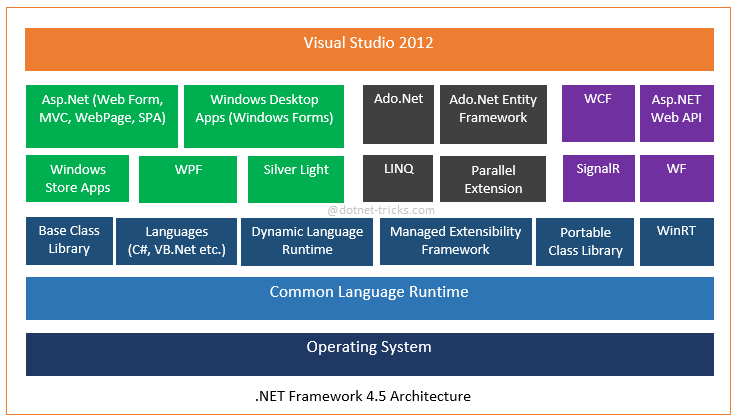
\includegraphics[width=140mm]{netframework45} 
\caption{Diagram som viser arkitekturen til .net rammeverket versjon 4.5} 
\label{fig:net-arkitektur} 
\end{figure} 
 
 
\section{Brukergrensesnitt-teknologi} 

Brukergrensesnitt-teknologi gir utvikleren tilgang på funksjoner og forhåndsdefinerte grafiske elementer som skal gjør utviklingen mer effektiv. Som en kan se utifra figur \ref{fig:net-arkitektur} og Microsoft's oversikt \cite{User1111:online} tilbyr .NET teknologier som Windows Store Apps, Windows Presentation Foundation(\gls{WPF}), Expression Blend 3 + SketchFlow, Windows Forms og Silverlight. Alle disse ble evaluert før et endelig valg ble foretatt:

\textbf{Windows Forms} ble utelukket ettersom dette er teknologien som Sono Flex er bygget på og som hadde begrensinger som gjorde at flere ønskede funksjoner ble vanskelig å implementere. 

\textbf{Windows Store Apps} hadde mye av den ønskede funksjonaliteten, samtidig som den fortsatt vedlikeholdes. Problemet var at for å distribuere slike applikasjoner brukes Windows Store. F å få publisert applikasjonen der, kreves godkjenning av Windows. En tidkrevende prosess. Dette i sammenheng med at disse applikasjonene ikke er kompatible med Windows 7\cite{Windo0:online} gjorde at denne teknologien ikke ble valgt. 

\textbf{Silverlight} er ifølge Microsoft sin blogg\cite{User1111:online} en kraftig utviklingsplattform for å lage "rike" media- og forretningsapplikasjoner for web, skrivebord og mobil. Fokus for teknologien er derimot på web og mobil \cite{Micro6:online}, og ettersom prototypen er en skrivebords applikasjon falt ikke valget på Silverlight.

Teknologien som til slutt ble valgt var \textbf{Windows Presentation Foundation}. WPF skal tilby utviklere en helhetlig programmeringsmodell for å bygge skrivebordsapplikasjoner for Windows som tar i brukergrensesnitt, media og dokumenter \cite{Windo777:online}. Grunnen til at teknologien ble valgt er:


\begin{itemize}
\item Fokus på skrivebord. I motsetning til blant annet Silverlight, er WPF designet og laget for å utvikle klient applikasjoner\cite{Windo777:online}.
\item Prioritert av Tobii PC Eye GO. I dokumentasjonen til øyesporingsenheten er det skrevet: "WPF  rammeverket er et svært bra verktøy for utvikling av grafikk-intensive applikasjoner og WPF har derfor blitt gitt høyest prioritet [..]"
\item Etterfølgeren til Windows Forms . Er ifølge Microsoft erstatteren til teknologien som blir brukt i Sono Flex \cite{User1111:online}. 
\item God støtte for animasjoner. WPF tilbyr blant annet et eget timing system for å enkelt holde tiden når en animerer grafiske elementer \cite{Anima7:online}.
\end{itemize}




 
\subsection{Windows Presentation Foundation} 
 
Ifølge Adam Nathan \cite[p.~9]{WPFbook}, programvare arkitekt hos Microsoft, ble prosessen med å lage WPF igangsatt fordi at mens grafisk maskinvare hele tiden har blitt bedre og billigere - samt at forbrukerens forventninger har fortsatt å stige, så var ingen som hadde adressert vanskeligheten med å lage moderne brukergrensesnitt.  

Han argumenterer med at det fantes utviklere på tiden som for eksempel brukte bitmap bilder til for å få et et annet utseende på for eksempel knappene enn det standardknappene hadde. Problemet er at disse formene for tilpasning ikke bare kan være ressurskrevende å utvikle, men også gi en dårligere brukeropplevelse. 

Han forteller videre at de ønsket å lage et rammeverk som hadde produktiviteten som folk likte med Windows Forms og som var enkel som HTML og Javascript.

WPF gir utvikleren mulighet til å utvikle applikasjoner med å bruke både markup språk og kode. Markup språket brukes vanligvis til å implementere utseende til applikasjonen, mens programmeringspråket brukes vanligvis til å implementere oppførselen. Det vil si at det er mulig å bruke de på tvers, men WPF legger opp til å skille mellom utseende og oppførsel \cite{Intro8:online}. Dette skillet skal ifølge utviklerene gi flere fordeler som blant annet reduksjon av utvikling og vedlikeholdskostnader ettersom utseende-spesifikk markup ikke er tett koblet med oppførsel-spesifikk kode. Det gir også designere mulighet til å jobbe med utseende samtidig som utviklere jobber med oppførsel \cite{Intro8:online}. I WPF er eXtensible Application Markup Language (XAML) brukt som markup språk. Mens man som programmeringspråk kan velge mellom C-Sharp eller Visual Basic.

\subsubsection{C-Sharp} 

Valget av programmeringsspråk sto mellom C-Sharp og Visual Basic (VB), to språk med svært forskjellig syntaks og historie \cite{Compa6:online}. C# har basert syntaksen sin på programmeringsspråket C , mens VB har sine røtter fra programmeringspråket BASIC \cite{Visua3:online} \cite{About8:online}. Begge språkene har de samme mulighetene, forskjellen ligger hovedsaklig i syntaks, så valget av programmeringsspråk ble basert på preferanser \cite{What0:online}. I dette tilfelle ble det valgt å ta i bruk C-Sharp, mye på grunn av likheten med Java som vi hadde erfaring med fra tidligere, men også på grunn dette var språket som ble mest brukt i eksempler og i dokumentasjonen til øyesporingenheten.


\subsubsection{eXtensible Application Markup Language (XAML)} 

XAML, en dialekt av XML, og har vært en viktig del av WPF siden dens introduksjonen i 2006 \cite[p.~17]{WPFbook}. Vanligvis brukes XAML til å spesifisere brukeregrensesnitt objekter og organiseringen av dem, men kan også brukes til andre ting som for eksempel animasjoner \cite{Story5:online}. 

Grunnen til at XAML har blitt brukt er fordi det er enkelt for programmere å samarbeide med eksperter fra andre felt. Nathan forteller at XAML blir felles språket for alle partiene, hovedsaklig gjennom utviklingsverktøy og felt-spesifikke design verktøy. Men også fordi XAML (og XML generelt) er enkelt å lese og forstå \cite[p.~17]{WPFbook}. Figur \ref{listing:knapp} viser hvor enkelt en kan genere en blå knapp som også er lettleselig .


\begin{listing}[ht] 
\inputminted[fontsize=\footnotesize, frame=lines,framesep=2mm,baselinestretch=1.2,bgcolor=lightgray,linenos]{xml}{Code/xamlexample.xml} 
\caption{Hvordan en blå knapp blir definert i XAML} 
\label{listing:knapp} 
\end{listing} 
 
   
\section{IDE og versjonskontroll} 

For å automatisere mye av utviklingen ble det valgt å bruke utviklingsmiljøet Visual Studio 2013 \cite{2013-1:online}. Grunnen til at Visual Studio ble valgt er det for at i tillegg til å ha kode-redigeringsverktøy og debugger, så har den også en WPF designer\cite{What8:online}. Denne designeren tilbyr flere hjelpemidler for å effektivisere prosessen med å lage brukergrensesnitt. Blant annet kan man velge mellom å kode de forskjellige elementene eller man kan dra dem inn fra et sidepanel. Den viktigste er derimot design vinduet, som til enhver tid viser hvordan brukergrensesnitt blir uten å måtte kjøre koden\cite{WPF D1:online}. 
 
For versjonskontroll ble det på grunn av erfaringsmessige årsaker brukt git\cite{AboutGit:online}. Til å ta backup av git filene ble den web-baserte tjenesten Bitbucket brukt. Grunnen til dette var at mye av koden fra Tobii Dynavox var konfidensiell og Bitbucket tilbyr gratis hemmelig oppbevaring. 
 
 
\section{Model View ViewModel} 

En viktig del av oppgaven var å bygge en prototype som Tobii Dynavox kunne bygge og teste videre på. Det var derfor en forutsetning at kildekoden var tilrettelagt for vedlikehold og videreutvikling. For å gjennomføre dette valgte vi å følge arkitekt mønsteret Model view Viewmodel (MVVM). Grunnen til at vi valgte dette fremfor mønster som for eksempel Model View Contoller(MVC)\{MVC a2:online} og Model-View-Presenter(MVP)/cite{The M4:online}. Er fordi MVVM ble utviklet av Microsoft spesifikk for å utnytte funksjonaliteten til WPF \cite{THEM6:online}. Artikkelforfatteren forteller videre at han ser på MVVM som skreddersydd for WPF. 

Det ble tidligere nevnt a WPF legger opp til å skille mellom utseende og oppførsel, MVVM skal hjelpe utviklere å følge dette prinsippet. Ved å skille mellom applikasjons logikk og brukergrensesnitt skal det ifølge Microsoft \cite{Im1online}, gjøre det enklere å teste, vedlikeholde og videreutvikle. MVVM gjør dette ved å dele opp koden i 3 deler - Modeller, ViewModel og View.
Figur \ref{fig:mvvm} viser de tre MVVM klassene view, view-model og model, og interaksjonen mellom disse.
 
\begin{figure}[ht!] 
\centering 
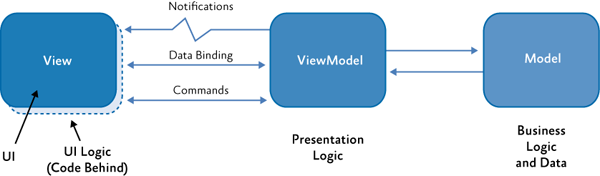
\includegraphics[width=100mm]{Mvvm} 
\caption{Illustrasjon som viser tre MVVM klasser og hvordan interaksjonen mellom dem\cite{Im1online}} 
\label{fig:mvvm} 
\end{figure}


\subsection{Modell}

Modell delen av MVVM står for en av de viktigste delene i enhver applikasjon, nemlig data og informasjon. Modellen sin eneste jobb er å representere og holde dataene som applikasjonen skal bruke. Den skal ikke hente data fra en database eller manipulere data på noen som helst måte \cite{Model7:online}. Dette går under forretningslogikk og skal ifølge mønsteret holdes separat fra modell-klasser. 


\subsection{View}
 
 Som navnet impliserer, skal klasser definert som View stå for visuelle elementer som vinduer, knapper, tekst, farger og organiseringen av dem. Med andre ord, selve brukergrensesnittet \cite{THEM6:online}. Grafiske objektet kan skrives ved hjelp av kode, men i MVVM skal alt som har med View og gjøre skrives XAML.
 
 

 
 
 For at en bruker skal kunne utføre kommandoer og hente data gjennom et view, brukes det i WPF, databindings uttrykk som blir evaluert opp mot viewets gitte datakontekst. I MVVM vil datakonteksten være satt til viewmodellen. Det vil si som figur \ref{fig:mvvm} viser, at alle former for kommandoer, notfikasjoner og databinding skjer gjennom viewmodellen. Et view vil typisk kun forholde seg til en viewmodel, altså et en-til-en relasjon\cite{.   
 
\subsection{ViewModell}
 
 ViewModellen er en nøkkelbrikke i MVVM 
 

The viewmodel is a key piece of the triad because it introduces Presentation Separation, or the concept of keeping the nuances of the view separate from the model. Instead of making the model aware of the user’s view of a date, so that it converts the date to the display format, the model simply holds the data, the view simply holds the formatted date, and the controller acts as the liaison between the two. The controller might take input from the view and place it on the model, or it might interact with a service to retrieve the model, then translate properties and place it on the view.

The viewmodel also exposes methods, commands, and other points that help maintain the state of the view, manipulate the model as the result of actions on the view, and trigger events in the view itself.

MVVM, while it evolved “behind the scenes” for quite some time, was introduced to the public in 2005 via Microsoft’s John Gossman blog post about Avalon (the code name for Windows Presentation Foundation, or WPF). The blog post is entitled, Introduction to Model/View/ViewModel pattern for building WPF Apps and generated quite a stir judging from the comments as people wrapped their brains around it.

I’ve heard MVVM described as an implementation of Presentation Model designed specifically for WPF (and later, Silverlight).

The examples of the pattern often focus on XAML for the view definition and data-binding for commands and properties. These are more implementation details of the pattern rather than intrinsic to the pattern itself, which is why I offset data-binding with a different color:
 
Mens viewet bestemmer hvordan applikasjonen skal se ut, så bestemmer viewmodellen hvordan funksjonaliteten skal være \cite{THEM6:online}. Det er i viewmodellen at egenskaper og kommandoer som viewet kan binde seg opp mot er implementert. Når data  da endres vil view bli varslet og oppdatert deretter(Notified i figur \ref{fig:mvvm}) . På samme måte vil viewet kalle på viewmodellen om at en kommando må kjøres hvis for eksempel en bruker trykker på en knapp. Det er også Viewmodellen sitt ansvar og koordinere interaksjoner med viewet med de modellene som trengs. Det vil si at viewmodellen kan eksponere modellen direkte til viewets slik at de kan bindingen kan skje direkte til dem. Samtidig kan viewmodellen også manipulere data fra modellen , som for eksempel å kombinere to verdier. Eksempel kan være å sette sammen fornavn og etternavn fra en Person modell. Mens forholdet mellom View og Viewmodellen typisk er en-til-en, så vil ViewModellen ha en en-til-mange relasjon.  
 
 
\subsection{MVVM light} 
 
 
//Siden ny utvikling og lage en testplattform, viktig at kode var optimalisert 
//Mvvm passet best skille mellom logikk og blablabla 
//Vikitg å få med design time data, side applikasjonen er svært design tung 
//Finn fordeler 
//mvvm light  - IOC container, design data. 
//Arkitektur 
 
 
 
\section{Utvikling}  
 
 
I seksjon \ref{sec:utgangspunk} ble teknologien som ble brukt til å utvikle prototypen diskutert. I denne seksjonen vil arkitektturen og de viktigste utviklingsdetaljene  bli drøftet.  
 
 
\subsection{Arkitektur} 
 
 
Figur \ref{fig:arkitektur} viser et forenklet bilde over hvordan klassene i kodebasen er koblet sammen. Med forenklet så menes det at flere hjelpeklasser og tredjeparts bilioteker er med i diagrammet. I tilegg så har ikke Views blitt tatt med i diagrammet, men for hver ViewModel så er det View som representerer det.  
 

\begin{figure}[ht] 
\centering 
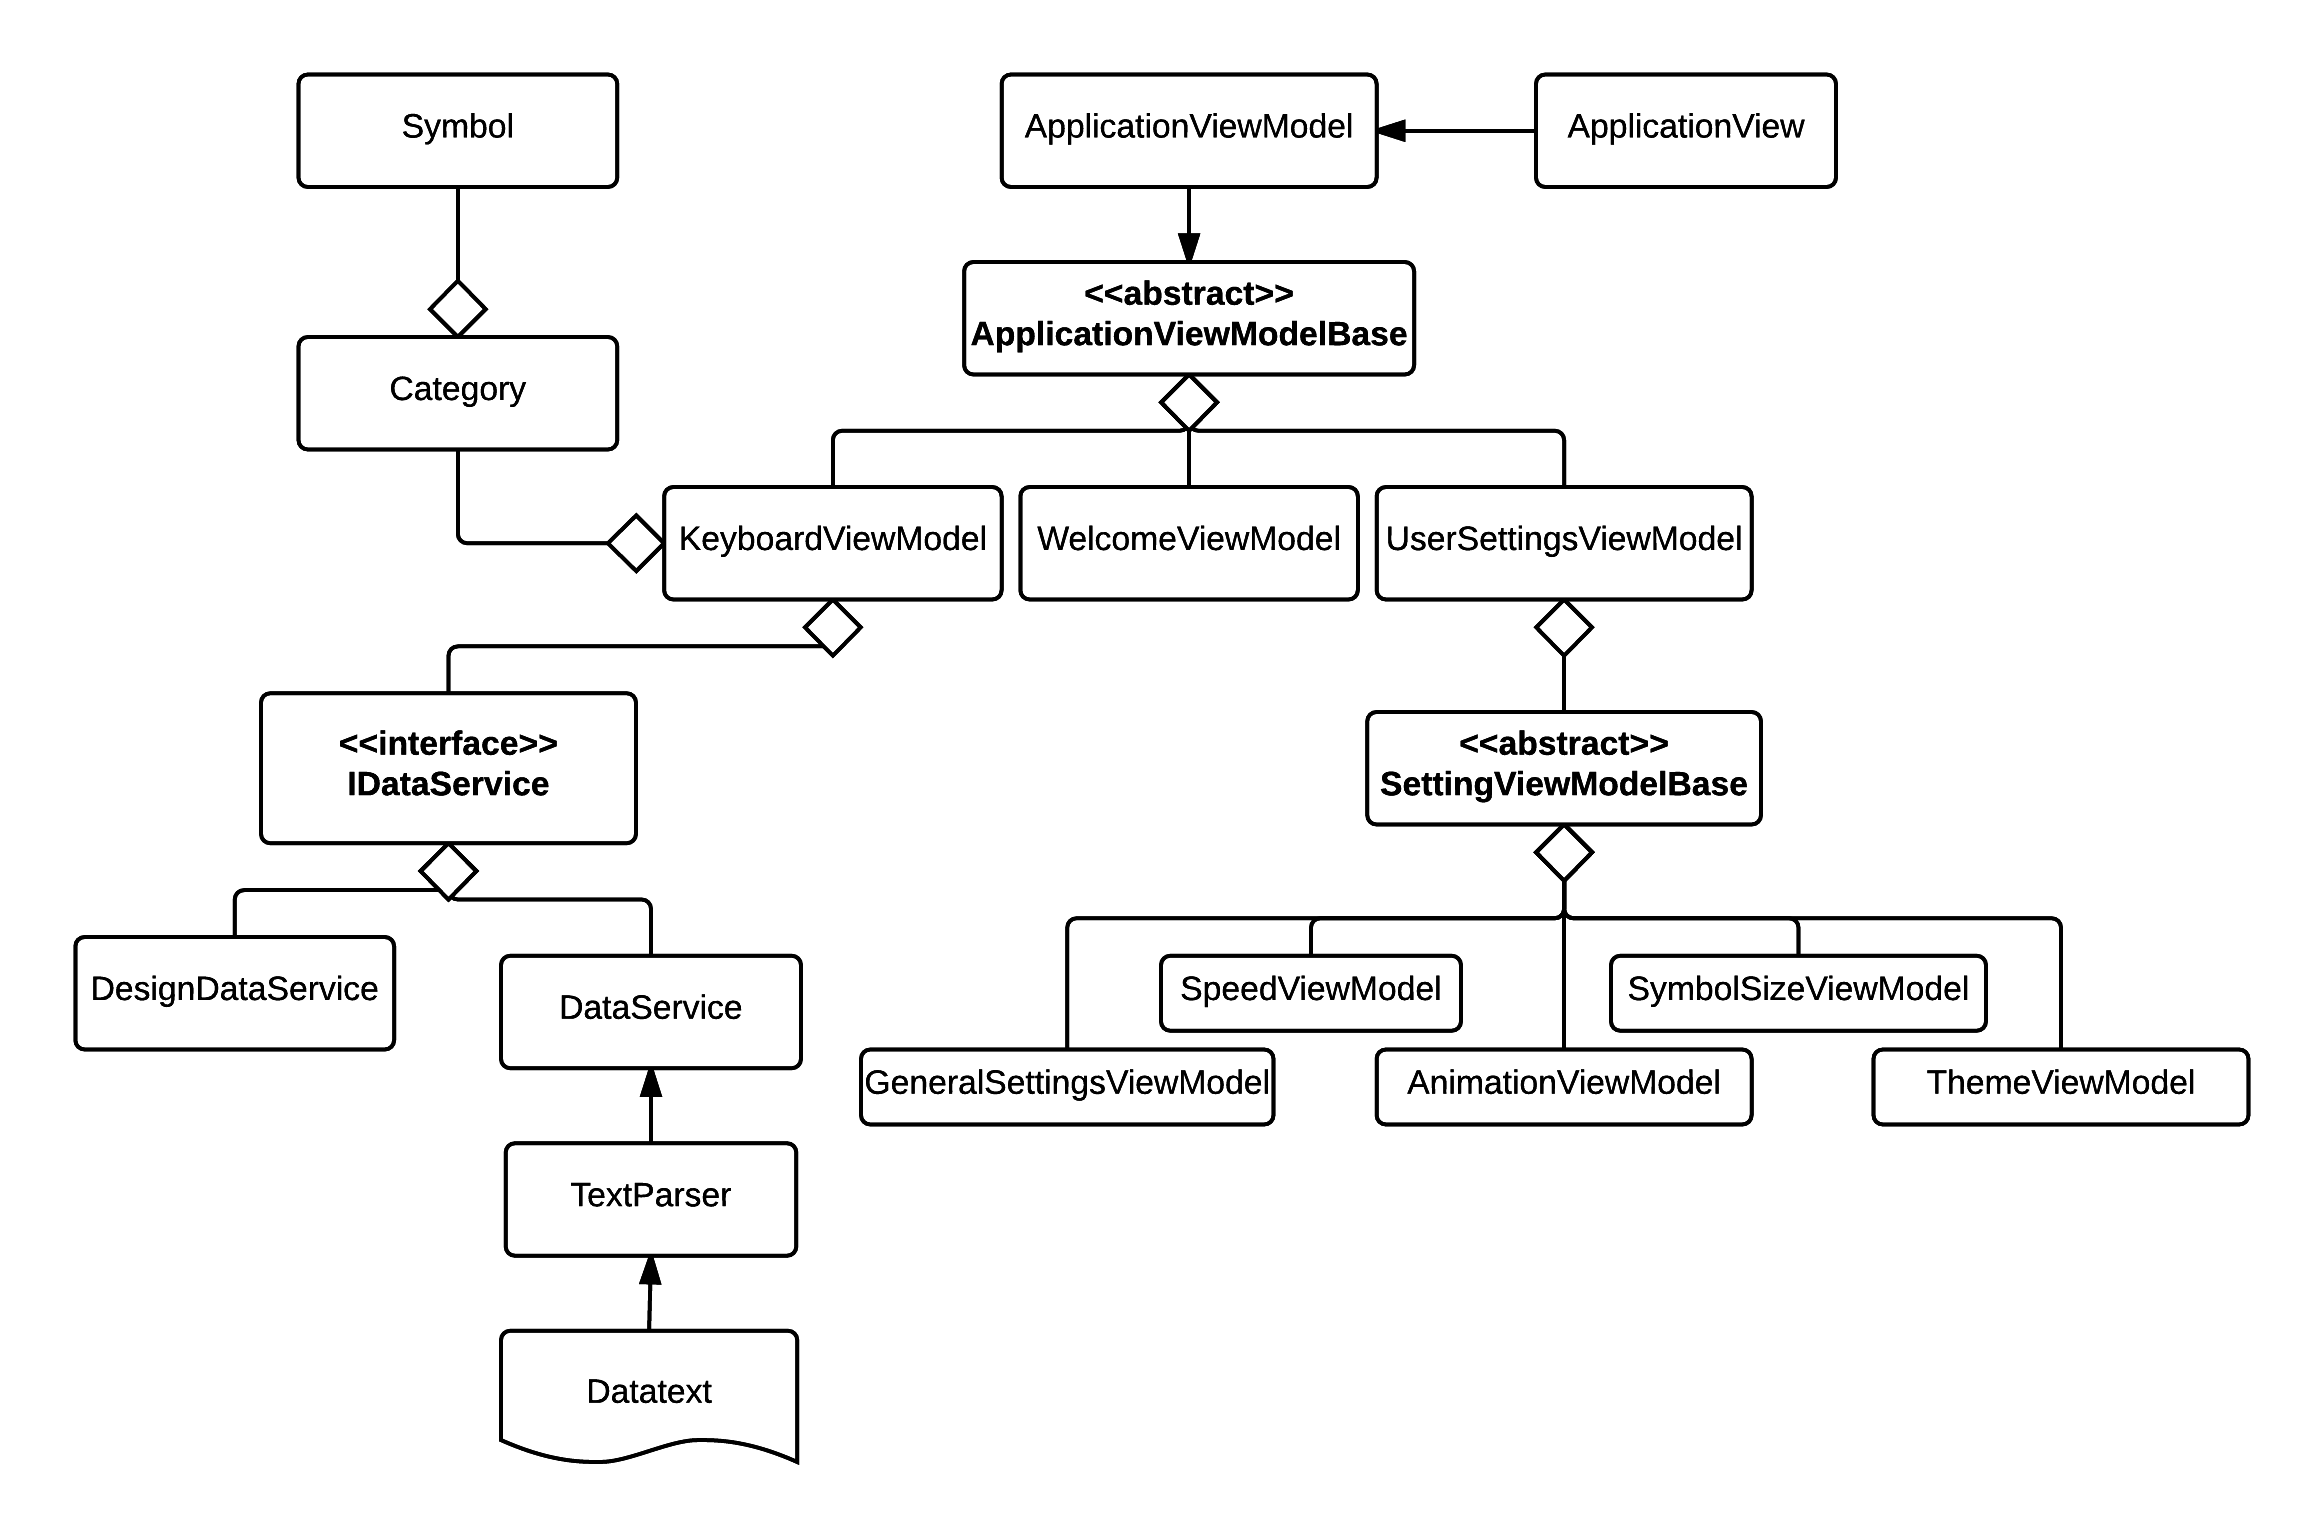
\includegraphics[width=140mm]{Arkitektur} 
\caption{Figur som viser et overordnet bilde av hvordan de ulike klassene henger sammen} 
\label{fig:arkitektur} 
\end{figure} 
 

 
ApplicationViewModel er vinduet som åpnes når programmet startes. Denne klassen fungerer som en kontainer for applikasjonen og bestemmer kun applikasjonsvinduets størrelse og navigasjon mellom de andre viewmodellene Keyboard, Welcome og UserSettings.  
 
 

\begin{listing}[ht] 
\inputminted[fontsize=\footnotesize, frame=lines,framesep=2mm,baselinestretch=1.2,bgcolor=lightgray,linenos]{xml}{Code/ApplicationContainer.xml} 
\caption{Utdrag fra kode som viser hvordan kontainer er satt opp} 
\label{listing:Kontainer} 
\end{listing} 
 
 
\begin{listing}[ht] 
\inputminted[fontsize=\footnotesize, frame=lines,framesep=2mm,baselinestretch=1.2,bgcolor=lightgray,linenos]{csharp}{Code/CurrentApplicationView.cs} 
\caption{Utdrag fra kode som viser hvordan kontainer er satt opp} 
\label{listing:CurrentAppView} 
\end{listing} 
 
 
 
Figur \ref{listing:Kontainer} viser hvordan ContentControl elementet i ApplicationView fungerer som en kontainer ved at innholdet er bundet til egenskapen CurrentViewModelBase. Som vil si at innholdet i ContentControl vil basere seg på hva som er satt som CurrentViewModelBase i ApplicationViewModel. Figur\ref{listing:CurrentAppView} viser hvordan denne egenskapen er implementert i Viewmodellen. Utfra koden så kan man se at til forskjell fra viewet, som hadde en referanse til egenskapen, så er det ingen direkte referanse fra viewmodellen til viewet. Dette er for å følge prinsippet til MVVM om at viewmodellen ikke skal ha noe kjennskap til Viewet, som gjør koden løs koblet(les: loose coupled). Men siden dette er en verdi som antakeligvis vil endre seg i løpet av kjøretiden er det nødvendig at Viewet blir gjort oppmerksom på forandring. Dette skjer ved å avfyre RaisePropertyChanged, dette kallet vil varsle rammeverket om at en endring har skjedd. Når da Viewet har en binding til denne egenskapen vil han bli oppmerksom på endringen og oppdatere deretter \cite{MVVM4:online}. 
 
CurrentViewModelBase er av typen ApplicationViewModelBase som vil si at det som er i kontaineren må være av nettopp denne typen. ApplicationViewModelBase er som man ser utifra figur  en abstrakt og har kun en abstrakt metode for å hente navn.  Det vil si at de klassene som arver fra ApplicationViewModel må implementere metoden. Fra figur kan man se at de klassene som arver fra ApplicationViewModel og med det har mulighet til å være i kontaineren er, KeyboardViewModel, UserSettingsViewModel og WelcomeViewModel. Sammen representerer disse hoved funksjonaliteten til programvaren. KeyboardViewModel er hoveddelen av applikasjonen, det her en bruker har mulighet til å skrive setninger med å trykke på de ulike symbolene for så å gjøre dem om til tale. I UserSettings kan en bruker se og endre på de ulike innstillingene. Mens \texttt{WelcomeViewModel} er kun laget for testingen og funksjonaliteten er begrenset til at en bruker kan velge alder og kalibrere øyesporingsenheten. 
 
 
 \subsection{Skrivebordet}
 
KeyboardViewModel og KeyboardView utgjør sammen det som blir kalt skrivebordet. Skrivebordet er den delen av programvaren som tilbyr hovedfunksjonaliteten, å la en bruker kunne skrive setninger. For å gjøre dette så må er det en del viktig elementer som må være tilstede. Man kan si at skrivebordet skal være en digital representasjon av det klassiske tastaturet. Der det er ord med symboler istedenfor bokstaver, og trykk skjer ikke ved fysisk trykk, men ved å se på knappen over en periode. Utenom dette skal funksjonaliteten være mye den samme. De mest nødvendige funksjonene som å kunne viske og bygge setninger må ihvertfall være tilstede. I tillegg må prototypen ha mulighet for å kunne presentere setningene som lyd. 

\begin{figure}[ht!] 
\centering 
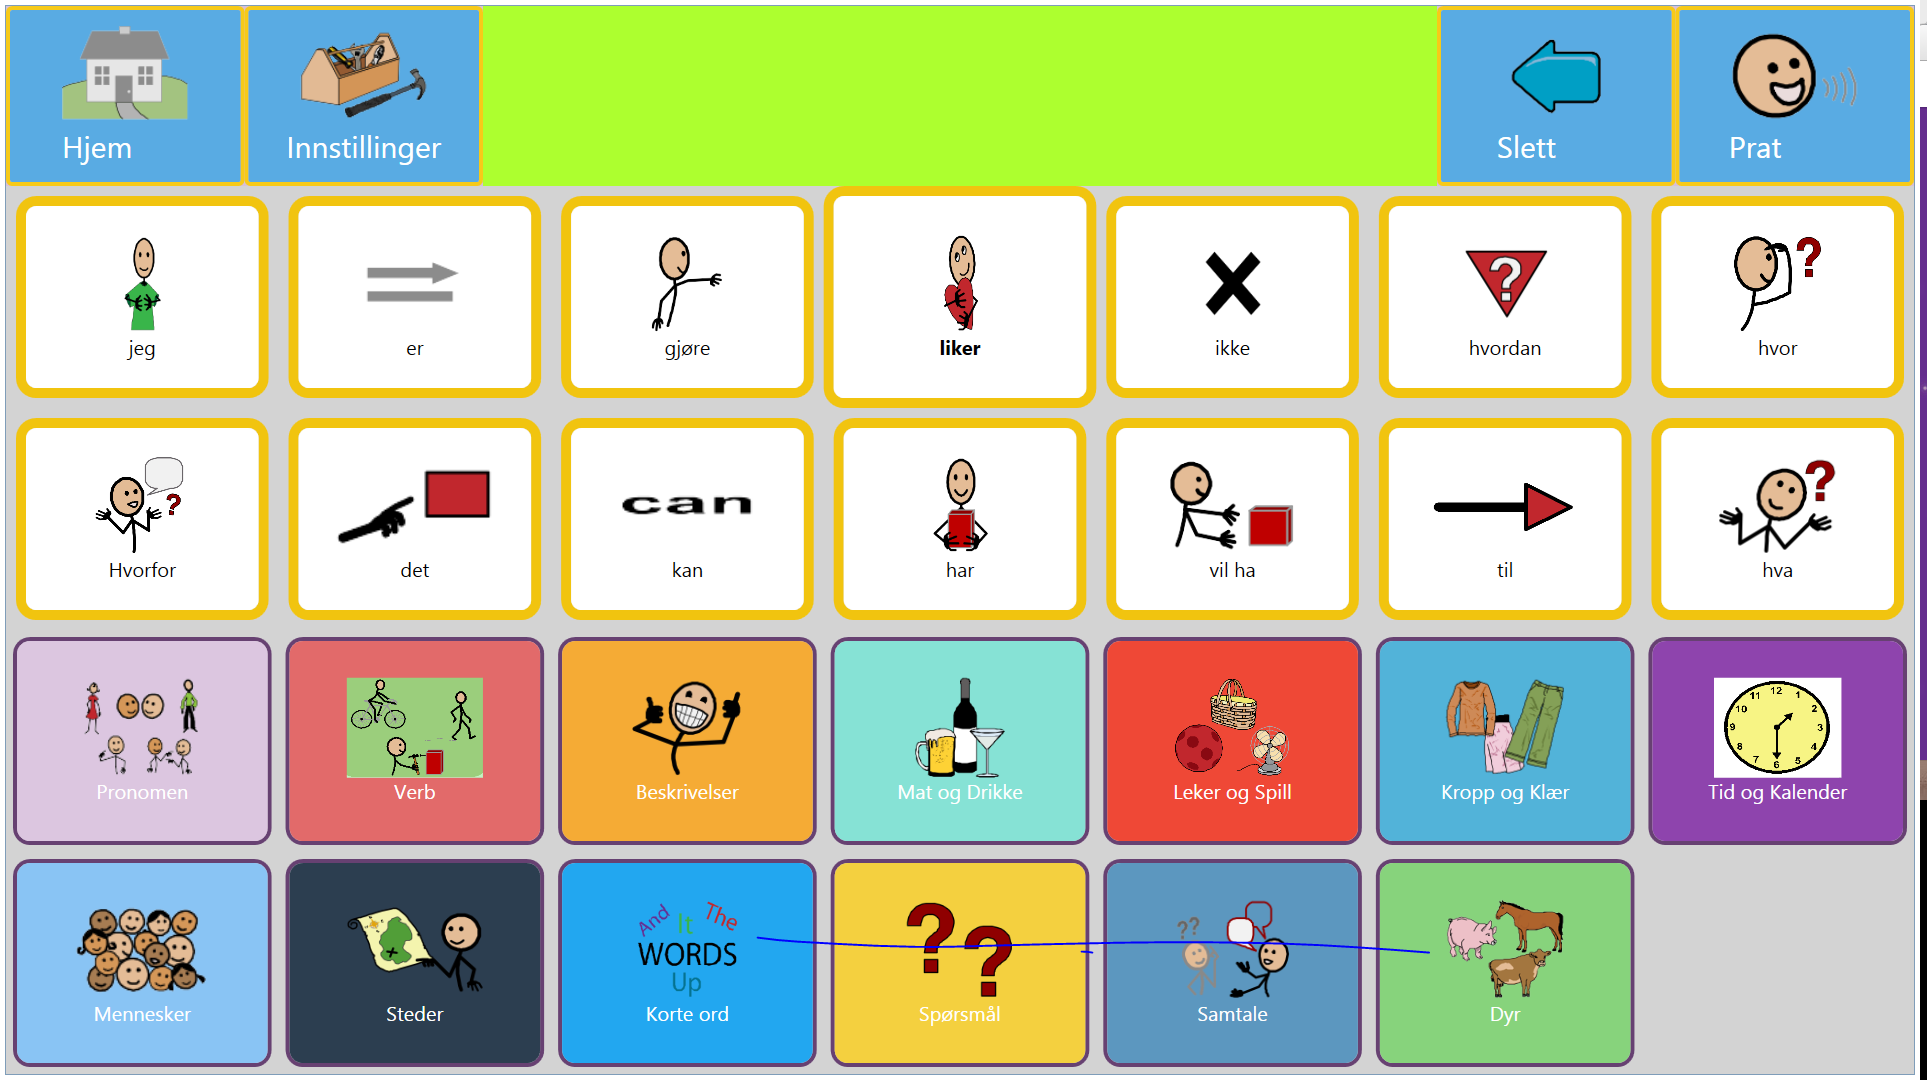
\includegraphics[width=100mm]{skrivebord} 
\caption{Skjermdump av skrivebordet i prototypen} 
\label{fig:skrivebord} 
\end{figure} 
 

\subsubsection{Innlesning}


For å kunne skrive med skrivebordet er det nødvendig at det er fullt opp med ord og symboler. For å gjøre dette blir metoden texttt{GetInitialPages} vist i figur .. kalt fra konstruktøren. Denne metoden kaller så igjen på metoden GetCategory("Frontpage") i klassen \texttt{Dataservice} vist i figur ... Grunnen til at ViewModellen ikke kun direkte henter symbolene er fordi de er lagret på et tekstdokument. Så for å separere data fra presentasjon- og forretningslogikk så brukes det et data tilgang lag i mellom. For å gjøre om tekstfilen til strukturerte data bruke datatjenesten klassen TextParser til å tolke den. 


\subsubsection{Data og innlesning av dem}

Programvaren skal strebe etter å kunne tilby brukeren ordene han har lyst å bruke. Noe som kan være utfordrende med tanke på at et barns vokabular allerede i alder av 5 år kan være opp i mot XXXX ord. Med tanke på hvilke ord som er i vokabularet vil variere  fra person til person så må programvaren ha en god del mer enn dette. I tillegg må også programvaren tilby et bilde for vært av ordene. 

En naiv fremgangsmåte for å lage brikkene er å statisk initialisere hver brikke med et ord og bilde. Problemet med dette er først og fremst at XAML koden blir unektelig lang som følge av at en må skrive en knapp for vært tilfelle. Den at en også må inn i koden for å gjøre endringer eller legge til nye ord, er ugunstig ettersom det er en ressurskrevende prosess. Løsningen på dette var å oppbevare alle ordene i en separat fil for å skille mellom brukergrensesnitt og data. For at maskinen skulle ha mulighet til å lese dataene ble de lagret i JavaScript Object Notation(JSON) format. JSON er ifølge sine egne nettsider \cite{JSON7:online} et lettvekt data-utvekslings format. Som er lett for mennesker å lese og skrive og det er lett form maskiner å tolke og generere. Kode \ref{listing:jsonfile} viser et utdrag fra json filen hvor ordene og stien til bildet som representerer ordet, er lagret. Filen består i en liste med JSON objekter som har attributtene Name og Image. Der Name er ordet og image er stien til symbolet. Dette er bare et lite utdrag fra filen og viser kun det som ville tilsvart fire brikker i programvaren. Det første objektet "I" er et ord, mens de tre neste er kategorier. Hver kategori består av flere ord. Ordene som tilhører en kategori er lagret i en egen fil i en mappe med samme navn. Figur \ref{jsonstructure} viser strukturen på filene, der hver kategori har sin egen mappe. Dette gjør at data hentes "just-in-time". Det vil si at istedenfor at ordene ligger i minnet til enhver tid, så hentes de kun når ved behov. Eksempelvis hvis en bruker trykker på kategorien "Food and Drink" så vil ordene hentes fra "FoodAndDrink.json" i mappen "FoodAndDrink". Noe som sparer på minnet, men som kan forringe kjøretiden. For når det er snakk om så store mengder data som alle ordene ville gitt, er det ikke gunstig å bevare dem i minnet. 


\begin{listing}[ht] 
\inputminted[fontsize=\footnotesize, frame=lines,framesep=2mm,baselinestretch=1.2,bgcolor=lightgray,linenos]{json}{Code/JSONfile.json} 
\caption{Utdrag fra filen som inneholder ord og sti til bilde som representerer det i JSON format} 
\label{listing:jsonfile} 
\end{listing} 
 
 
 \begin{figure}[ht!] 
\centering 
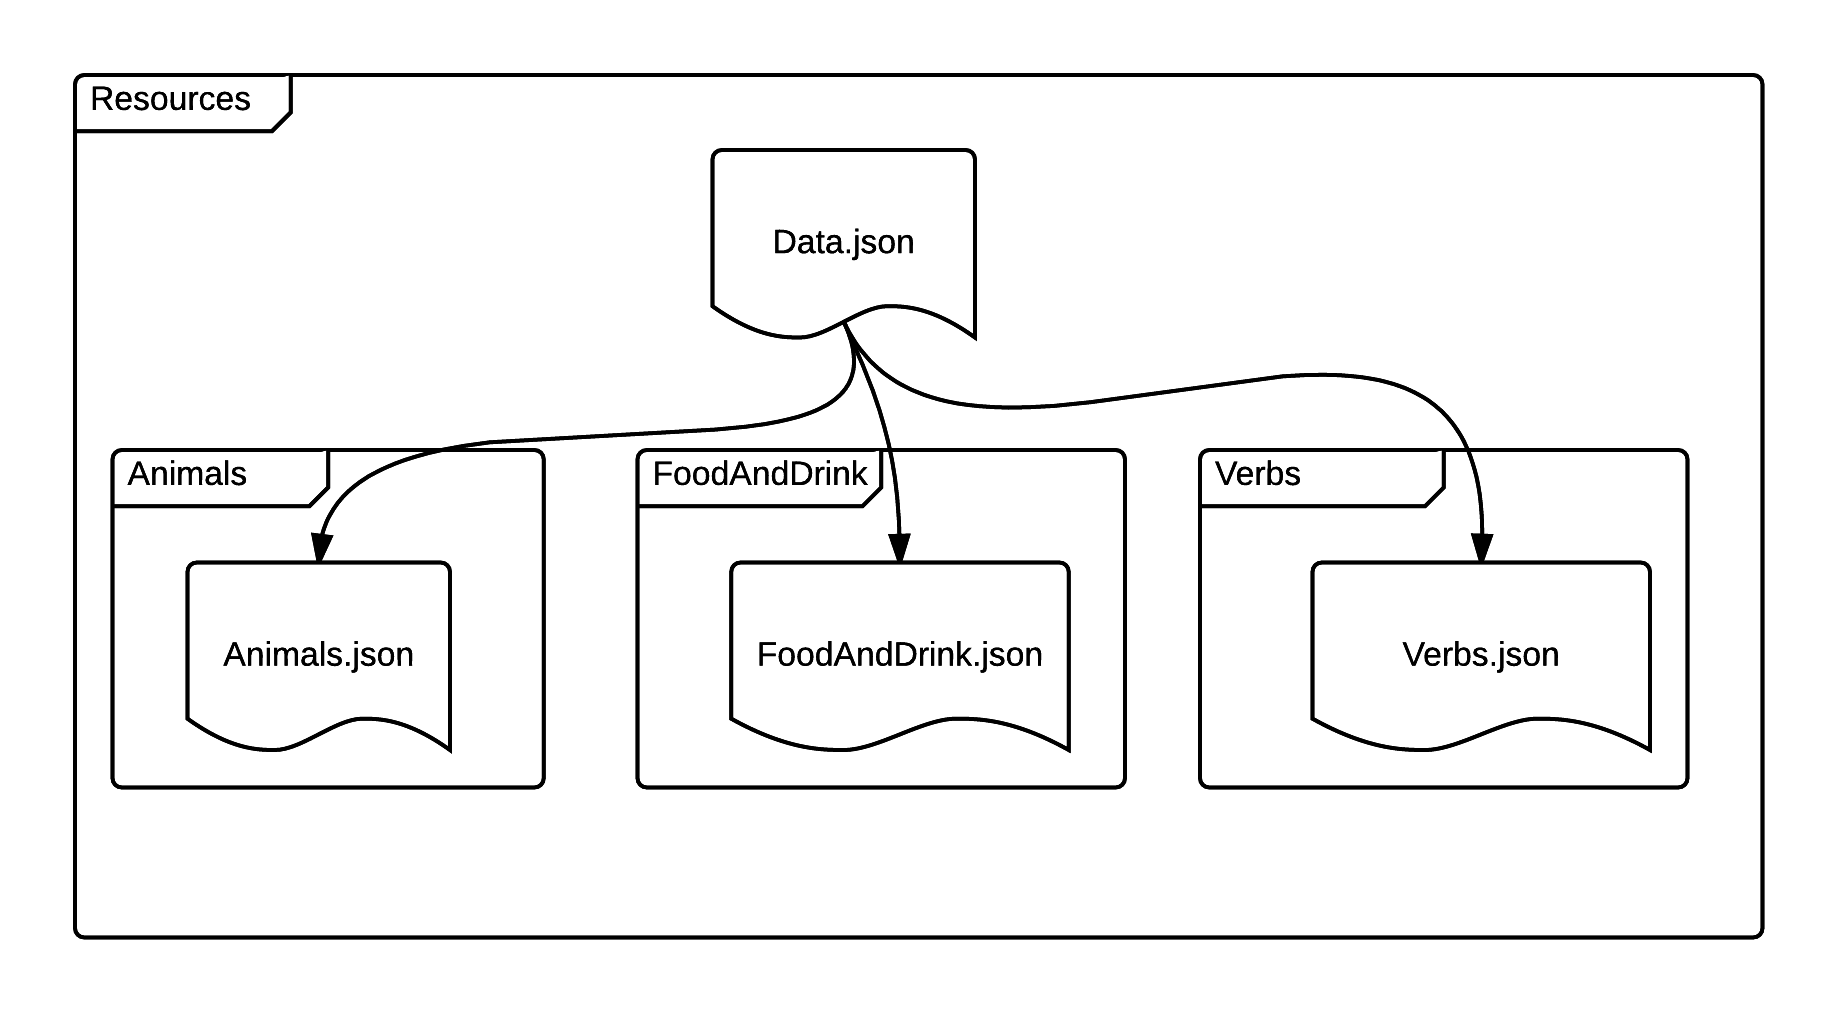
\includegraphics[width=100mm]{JsonStructure} 
\caption{Bilde av dokumentet hvor de ulike symbolene er registrert} 
\label{fig:jsonstructure} 
\end{figure} 


For å kunne ta i bruk objektene definert i tekstfilen må de tolkes fra JSON format til .NET objekter. Denne prosessen, å trekke ut datastrukturer fra bytes, kalles deserialisering. For å gjøre dette har vi brukt et tredjeparts rammevekt kalt JSON.net \cite{Json.0:online}. Det finnes en innebygd funksjon i .NET kalt DataContractJsonSerializer \cite{DataC3:online} som også greier å deserialisere et JSON dokument. Grunnen til at JSON.NET ble brukt er fordi i dette biblioteket er det mulighet for å automatisk deserialisere en helt liste av JSON objekter til .NET liste uten å manuelt måtte legge inn objektene. Ifølge utviklerens egne nettsider skal rammeverket være 50 prosent kjappere enn DataContractJsonSerializer, men ytelsen er avhengig av hvilke datasett som brukes, og har ikke vært en faktor i avgjørelsen. 


\begin{listing}[ht] 
\inputminted[fontsize=\footnotesize, frame=lines,framesep=2mm,baselinestretch=1.2,bgcolor=lightgray,linenos]{csharp}{Code/JSONparser.cs} 
\caption{Koden som konverterer JSON filen til en IList} 
\label{listing:JsonParser} 
\end{listing} 


Koden i figur \ref{listing:JsonParser} deserialiserer JSON dokumentet om til en dataliste. Fra linje 5 til 12 skrives teksten fra filen over til en streng som kan manipuleres i koden. På linje nummer 14 blir strengen konvertert til et dataobjekt. Det at dokumentet blir gjort om fra streng til et komplekst objekt på kun en linje viser noe av styrken til json.NET. 

\begin{listing}[ht] 
\inputminted[fontsize=\footnotesize, frame=lines,framesep=2mm,baselinestretch=1.2,bgcolor=lightgray,linenos]{csharp}{Code/CategoryModel.cs} 
\caption{Category modellen har egenskapen navn og en liste over alle sidene som utgjør alle symbolene som hører til i kategorien} 
\label{listing:CategoryModel} 
\end{listing} 


\subsection{Teksttolker}

Under utviklingen ble det bare lagt inn tilfeldige ord i prototypen, men ettersom prototypen begynte å bli ferdigstilt var det behov for et større utvalg ord og symboler Det ble derfor gitt tillatelse av Tobii Dynavox til å ta i bruk det samme bildene som de bruker i deres programvare. Denne bildepakken heter SymbolStix og har gir tilgang på cirka 16 000 symboler og er levert av et eksternt selskap som heter n2y \cite{n2y}. 

\begin{itemize}
\label{itm:egenskaper}
\item Symbol ID
\item Dato oppdatert
\item Dato laget
\item Kategori Navn 
\item Filnavn
\item Filsti
\item Ord
\item Synonymer
\item Tysk, nederlandsk, norsk, svensk, dansk, engelsk, spansk, italiensk, fransk, portugisisk.
\end{itemize}


Sammen med bildepakken fulgte det med et dokument som hadde en beskrivelse av vært symbol. For vært symbol var egenskapene beskrevet i liste \ref{itm:egenskaper} tilgjengelig. Disse var strukturert med at de kom i rekkefølge og hadde tilde notasjon(tilde) for å skille mellom dem. Dette gjorde at det var mulig å implementere en løsning for å gjøre dem om til datastrukturer. I tillegg til å tilby det samme som JSON dokumentet, ord og bildesti, så har den også ordets kategori og synonymer for ordet. Det er også mulighet for å få ordet på flere språk og synonymer til de ulike språkene. Noe som åpnet for flere muligheter, men for å få til dette, måtte det legges til en annen form for innlesing av data ettersom dokumentet ikke var lagret i JSON format og I motsetning til å dele opp symbolene opp i separate dokumenter basert på hvilken kategori de tilhørte, så var alle deklarert på et dokument. Så for å kunne løse dette sto vi mellom å lage et skript som oversatte dokumentet til JSON format eller lage en alternativ innlesning. Å omgjøre det fra tekst til JSON hadde vært mulig, problemet med dette er at dokumentet utsatt for oppdatering. Så hver gang dokumentet blir forandret må oversetting gjøres på ny. Så det ble da bestemt for å implementere en teksttolker. 

Tekstolkeren er er mer kompleks enn JSON tolkeren. Hovedsaklig fordi det ikke finnes noe biliotek som automatisk tilegner egenskaper til symbolene. Egenskapene blir derfor gitt til vært symbol etterhvert som de blir lest inn. En annen utfordring var som tidligere nevnt at alt befant seg på et dokument som da totalt utgjorde 16 000 linjer med beskrivelse av symbolene. Slik at hvis en skulle ha brukt samme fremgangsmåte som med JSON parseren å kun lest inn for den gitte kategorien. Så hadde en i verste fall måtte ha lest 16 000 linjer med tekst. Dette er ikke gunstig. Dokumentet har flere kategorier og symboler som ikke er nødvendig for barn, blant annet egne kategorier som eksempel Brasil, hebraisk og sveitsisk. Det er også flere kategorier som kunne vært greit å ha, men som ikke prioriteres som blant annet kategorier om kjendiser og en egen om amerikanske byer. Det ble derfor bestemt å kun velge kategorier som var nødvendige.

\begin{figure}[ht!] 
\centering 
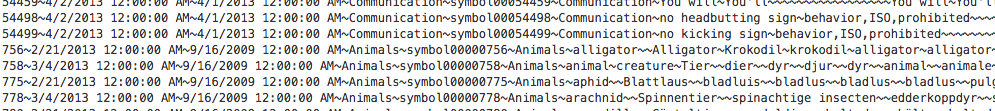
\includegraphics[width=100mm]{datafil} 
\caption{Bilde av dokumentet hvor de ulike symbolene er registrert} 
\label{fig:dok} 
\end{figure} 


\subsection{Modellene}

Modellene i MVVM mønsteret enkapsulere forretningslogikk og data. Der forretninslogikk er definert som all applikasjonslogikk med tanke på innhenting og håndtering av applikasjonsdata for forsikre seg om at data er konsistent og validering er pålagt. Bruk av modeller skal hjelpe til med å maksimere gjenbruk.

I applikasjonen er det flere modeller, men det som blir brukt mest er Symbol modellen. Denne representerer alle data i symboltabellen. Der det blant annet er et bilde og et ord som representerer dette bildet. Den har også egenskaper som forteller om hvilken type knapp det er, altså navigering,kategori eller ord. Hvilken knapp det er vil påvirke hva som skjer når en bruker interagere med denne.



\section{SymbolStix} 
 
En viktig del av programvaren er å hjelpe barn å bygge et vokabular ved å visualisere ord med bilder. Det vil si at for hvert ord må det finnes et bilde, noe som kan bli svært mange. Tobii Sono Flex har løst denne oppgaven med å bruke et kommersielt tredjeparts bildebibliotek kalt SymbolStix \cite{n2y}, utviklet av n2y. Bildene i biblioteket består av svært enkle tegninger som kun har med det mest nødvendige får å få frem konseptet eller ordet symbolet prøver å representere. Det at Sono Flex og at dette bildebiblioteket var tilgjengelig gjennom Tobii gjorde at den samme bildepakken skulle bli brukt i prototypen. Dette gjorde også medføre at ikke unødvendig med ressurser ble brukt på anskaffe bilder for hvert ord. 
 
 
\section{Utfordringer}

\subssection{Problem} 
 
Symbolstix bildene er lagret i Enhanced Metafile Fomat (EMF), som er et 32-bit format som kan inneholde både vektor og bitmap informasjon\cite{AboutEMF}. Problemet med EMF formatet er at det ikke finnes støtte for dette i WPF, med den begrunnelse at det har blitt funnet en kritisk sårbarhet\cite{EMFVulnerability} og at formatet er mer mottakelig for sårbarheter\cite{EMFForum} enn andre bildeformater. I Sono Flex fungerer dette fint, fordi det bygget på Windows Forms(WF),  et rammeverk som har innlagt støtte for EMF. WPF har støtte for å bruke WF elementer,  en funksjon som ble lagt inn for å lette overgangen fra WF til WPF. Som igjen gjorde det mulig å hente bilder med EMF format. Ulempen er at man må trekke inn store deler av WF biblioteket noe som fører til en betraktelig økning i størrelse. For å aktivere støtten, deklarerer en WindowsFormHost i xaml filen og denne vil fungere som en kontainer for alle WF elementer. Innenfor denne kontaineren vil alt fungere som i et WF miljø. Ved å gjøre dette ble alle bildene hentes og vist i prototypen.  
 
 
Testing av applikasjonen viste derimot at det ikke lenger var mulig å trykke på knappene, eller mer korrekt, det var ikke mulig å trykke på  bildet der knappen var. Dette viste seg å være kjent problem, og er kjent som Airspace problemet (kilde) og kommer av at alle WF elementer uansett vil legge seg over alle WPF elementer. Et problem som ikke kunne være med i prototypen. En fix til dette ble laget og planlagt lansert i .NET versjon 4.5, men da versjonen ble lansert, var ikke denne fiksen med. Det finnes ulike omveier rundt på problemet, men få tilfredsstillende.  
 
 
Det ble derfor prøvd å konvertere EMF filene til bitmap for så å vise de i applikasjonen. Fordelen med denne fremgangsmåten var at vi slapp å trekke inn windows forms biblioteket. Ulempen var derimot at hver gang et symbol skulle hentes så måtte dette først konverteres til Bitmap for deretter og rendres. En tidkrevende prosess som gjorde at det tok flere sekunder å laste brukergrensesnittet. Det ble derfor prøvd å konvertere alle filene og deretter lagre dem som jpg. Konverteringen ville da kun gjøres en gang. Deretter ville applikasjonen hente jpg filene direkte, uten noe omvei. Siden wpf har innebygd støtte for formatet. Igjen viste det seg at dette ikke var godt nok ettersom jpg filene hadde blitt for store i overgangen fra vektor til raster grafikk og de manglet gjennomsiktighet. For mens EMF filene lå på under 10kb endte alle de konverterte filene opp på over 100kb. Noe som i selv ikke er så stort, men som gir utslag på lastingen av applikasjonen når det kan være opp mot 200 bilder som skal lastes. 
 
 
Den endelig løsningen ble å laste ned et profesjonelt konverteringsverktøy kalt AVS Image converter. En svært ømfintlig prosess som tok svært lang tid, men som gjorde det mulig å konvertere de orginale EMF filene til png og samtidig holde størrelsen på rundt 10 kb. 


\subsection{Sette seg inn i teknologiene}

\subsection{Følge MVVM mønsteret}
 
 
\section{Applikasjonen} 

Prototypen har den samme layouten som Tobii Sono Flex, med en menylinje etterfulgt av en symboltabell under. Det er derimot en del variasjoner inne i hver av disse komponentene. 
 
 
\subsection{Menylinjen} 
 
Menylinjen dekker 1/5 del av applikasjonens vindu og består av 4 knapper og listen over ord som brukeren har trykket på. Denne listen vil heretter bli referert til som ordlisten. 
 
 
\subsubsection{Tilbaketasten} 
 
Tasten som befinner seg til høyre for ordlisten er tilbake tasten. Som på et vanlig tastatur vil et trykk på denne knappen medføre at det siste ordet i ordlisten fjernes. 
 
 
\subsubsection{Ordlisten} 
 
Når en bruker trykker på et ordsymbol så vil dette legge seg i ordlisten og når han trykker på "prate" knappen så vil ordene i listen bli gitt gjennom høyttalerne som naturlig tale og deretter fjernes fra listen. Selv om det er plass til uendelig med ord i listen så vil det kun være mulig for brukeren å se maks 4 om gangen. Hvis det allerede er fire symboler i listen når brukeren trykker på et nytt symbol, så vil de tre første bli "fjernet" mens det fjerde og det nye symbolet vil være igjen. Hvis brukeren igjen fjerner de to siste ordene ved å trykke på tilbaketasten,  vil ordene som kommer før igjen bli presentert for brukeren i setningsliseten.  
 
 
\subsubsection{Hjem} 
Ved å trykke på "hjem" knappen vil brukeren alltid bli ført til førstesiden av applikasjonen uavhengig av hvor han befinner seg.  
 
 
\subsubsection{Innstillinger} 
Hvis brukeren første er på "hjem" siden av applikasjonen så vil knappen byttes ut med en "innstillinger" knapp. Ved å trykke på denne vil det åpnes et nytt vindu hvor brukeren vil ha mulighet til å sette og endre på diverse innstillinger. Detaljene rundt denne siden er beskrevet i seksjon. 
 
 
\begin{figure}[ht!] 
\centering 
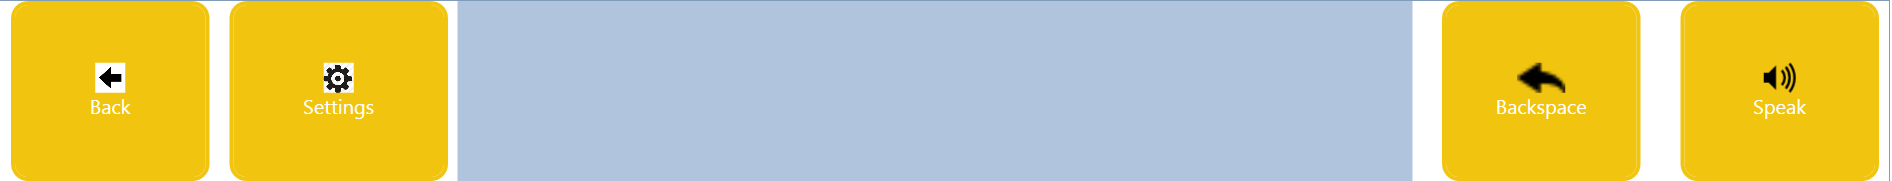
\includegraphics[width=100mm]{MenylinjeP} 
\caption{Skjermdump av menylinjen i prototypen} 
\label{fig:menylinjen} 
\end{figure} 
 
 
\section{Symboltabellen} 
 
 
Symboltabellen består av like mange kolonner og rader som den gjør i Sono Flex,  men det er måten den oppfører seg på som er annerledes.   
 
 
\section{Sammendrag} 

Kapittelet forklarer hvordan prototypen fungerer og prosessen med å utvikle den. Prototypen har blitt implementert med en moderne teknologi som fortsatt er støttet. Det har blitt lagt vekt på kodekvalitet under utviklingen. Blant annet så har vi følgt et design mønster som passer bra både til teknologien og plattformen som den skal kjøre på. Alle kravene satt i kravspesifikasjonen har blitt implementert, men noen ikke i like stor grad som ønsket. 

